\begin{tikzfigure}
\centering

\def\scl{0.45} % define scale variable for plots

\begin{tikzpicture}
% Diagram and plot
\matrix [row sep=0.25cm, column sep=0cm, style={align=center}] (my matrix) at (0,0)
{

\node[anchor=center] (diagram) {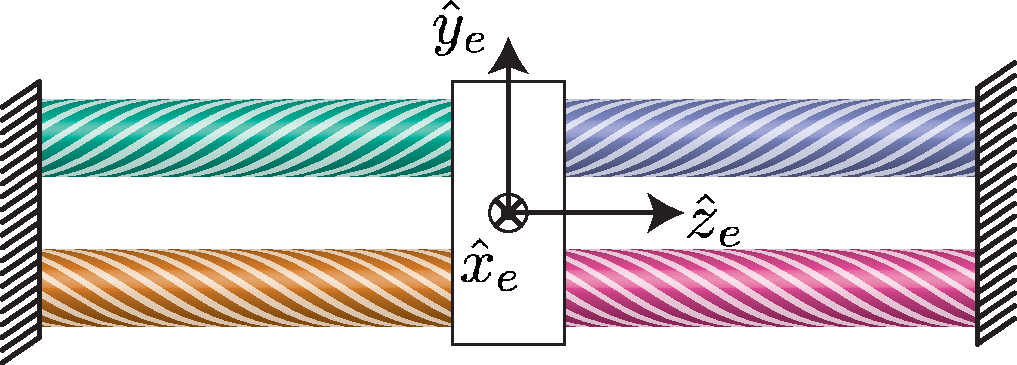
\includegraphics[width=\linewidth]{images/zntpExampleRig4.pdf}};

\\

\begin{axis}[
    view={90}{0},
    axis lines=center,
    % axis equal image,
    xlabel={$M^{\hat{x}_e}$},
    ylabel={$F^{\hat{z}_e}$},
    zlabel={$M^{\hat{z}_e}$},
    ymin=-7, ymax=7, ytick={0}, %ylabel near ticks,
    xmin=-5, xmax=10, xtick={0}, %xticklabel=$\pgfmathprintnumber{\tick}^\circ$, xlabel near ticks, 
    zmin=-7, zmax=7, ztick={0}, %z dir=reverse,
    xlabel style={anchor=north}, ylabel style={anchor=north},
    % scale=\scl,
    anchor=center,
    name=plot4,
    width=\linewidth,
    height=5.25in,
    line width=5pt,
    ]
    \def\pa{(-2,-3,2)}
    \def\pb{(2,-3,-2)}
    \def\pc{(2,3,-2)}
    \def\pd{(-2,3,2)}

    % connector lines for perspective
    \addplot3[dotted, line width=2pt] coordinates {(0,0,0) (-2,-3,0)};
    \addplot3[dotted, line width=2pt] coordinates {(-2,-3,0) \pa}; 
    \addplot3[dotted, line width=2pt] coordinates {(0,0,0) (2,-3,0)};
    \addplot3[dotted, line width=2pt] coordinates {(2,-3,0) \pb};
    \addplot3[dotted, line width=2pt] coordinates {(0,0,0) (2,3,0)};
    \addplot3[dotted, line width=2pt] coordinates {(2,3,0) \pc};
    \addplot3[dotted, line width=2pt] coordinates {(0,0,0) (-2,3,0)};
    \addplot3[dotted, line width=2pt] coordinates {(-2,3,0) \pd};
    % faces of shape
    \addplot3[patch, opacity=0.3, fill=black!20, faceted color=black, patch type=rectangle, line width=1pt] 
        coordinates {
                    (0,0,0) \pa (0,-6,0) \pb
                    (0,0,0) \pb (4,0,-4) \pc
                    (0,0,0) \pc (0,6,0) \pd
                    (0,0,0) \pd (-4,0,4) \pa
                    };
    
    % force vectors for each FREE                
    \addplot3[->, line width=5pt, plgreen] coordinates {(0,0,0) \pa};
    \addplot3[->, line width=5pt, plorange] coordinates {(0,0,0) \pb};
    \addplot3[->, line width=5pt, plpurple] coordinates {(0,0,0) \pc};
    \addplot3[->, line width=5pt, plpink] coordinates {(0,0,0) \pd};
\end{axis};

\\
};

\end{tikzpicture}
    
\end{tikzfigure}